\documentclass[aspectratio=169]{beamer}
\usetheme{Madrid}
\usefonttheme{structurebold}
\usefonttheme[onlymath]{serif}

\definecolor{BKTemplate}{rgb}{0.11765, 0.30588, 0.47451}
\usecolortheme[named=BKTemplate]{structure}
\setbeamercolor{title}{fg=BKTemplate,bg=}
\setbeamertemplate{caption}[numbered]
\setbeamertemplate{navigation symbols}{}
\setbeamertemplate{footline}[frame number]

\usepackage[utf8]{inputenc}
\usepackage[T5]{fontenc}
\usepackage{lmodern}
\usepackage{url}
\usepackage{booktabs}
\usepackage{graphicx}
\usepackage{array}
\usepackage{multirow}
\usepackage{amsmath}
\usepackage{amsfonts}
\usepackage{microtype}
\usepackage{pifont}
\usepackage{xcolor}
\usepackage{tikz}
\usetikzlibrary{positioning, arrows.meta, calc}

\graphicspath{{images/}{images/dashboard/}{images/analysis/}{../report/img/}{../report/img/dashboard/}{../report/img/analysis/}}

% Khoảng cách ô thống nhất cho bảng kiểu ``khung kín'' (|...| + \hline)
\newcommand{\slideTablePad}{%
  \setlength{\tabcolsep}{7pt}%
  \renewcommand{\arraystretch}{1.25}%
}

%------------------------------------------------------------
% Title page configuration
%------------------------------------------------------------
\title[Xây dựng Airline DW]
{\vspace*{0.5cm}\\\textbf{\large BÁO CÁO BÀI TẬP LỚN}}

\subtitle{\textbf{\Large XÂY DỰNG KHO DỮ LIỆU VÀ KHAI PHÁ DỮ LIỆU\\CHO LĨNH VỰC HÀNG KHÔNG}}

\author[Nhóm 2211322-2211337-2210429]
{\textbf{GVHD:} Thầy Đỗ Thanh Thái\\
\vspace{0.2cm}
\textbf{SVTH:} Đoàn Trí Hùng (2211322); Nguyễn Mạnh Hùng (2211337);\\
Nguyễn Cao Cường (2210429)}

\institute[HCMUT]
{
  Khoa KH\&KT Máy tính
}

\date[Apr 2026]
{Tháng 4, 2026}

%------------------------------------------------------------
% Auto-insert TOC at the beginning of each section
%------------------------------------------------------------
\AtBeginSection[]
{
  \begin{frame}
    \frametitle{Nội dung chính}
    \tableofcontents[currentsection]
  \end{frame}
}

\begin{document}

% --- Title page (with front background) ---
% --- Title page (with front background) ---
\setbeamertemplate{background canvas}{%
	
\includegraphics[width=\paperwidth,height=\paperheight]{images/FrontBackground.pdf}%
}

\begin{frame}[plain]
\titlepage
\end{frame}

% --- Set background for all remaining pages ---
\setbeamertemplate{background canvas}{%
	
\includegraphics[width=\paperwidth,height=\paperheight]{images/Background.pdf}%
}

% --- Phân chia công việc ---
\begin{frame}
\frametitle{PHÂN CHIA CÔNG VIỆC}
\begin{itemize}
    \item \textbf{Đoàn Trí Hùng (2211322):}
    Xây dựng pipeline ETL, thiết kế Star Schema (SQLite),
    phát triển Dashboard Streamlit 6 trang,
    viết báo cáo. (100\%)

    \item \textbf{Nguyễn Mạnh Hùng (2211337):}
    Huấn luyện và so sánh 5 mô hình ML
    (Logistic Regression, Random Forest, Neural Network,
    XGBoost, LightGBM),
    phân tích kết quả, Feature Importance. (100\%)

    \item \textbf{Nguyễn Cao Cường (2210429):}
    Khảo sát dữ liệu nguồn,
    xây dựng bộ truy vấn OLAP,
    tổng hợp tài liệu tham khảo, làm slide thuyết trình. (100\%)
\end{itemize}
\end{frame}

% --- Table of contents ---
\begin{frame}
\frametitle{Nội dung chính}
\tableofcontents
\end{frame}

% ================= SECTION 1: BÀI TOÁN =================
% ============================================================
% SECTION 1: BÀI TOÁN
% ============================================================
\section{Bài toán}

% --- Slide 1 ---
\begin{frame}{Bối cảnh}
\begin{columns}[T,onlytextwidth]
\begin{column}{0.5\textwidth}
\begin{itemize}
  \item Năm 2015: khoảng \textbf{5,8 triệu} chuyến bay nội địa Hoa Kỳ.
  \item Tỷ lệ đáng kể trễ đến $\geq 15$ phút,
        gây chi phí vận hành và giảm trải nghiệm hành khách.
  \item Phân tích thủ công (Excel, SQL rời rạc) \textbf{khó mở rộng},
        không phát hiện được pattern ẩn.
\end{itemize}

\vspace{2mm}
\begin{alertblock}{Nhu cầu}
Cần một hệ thống tích hợp: tự động hóa dữ liệu, phân tích đa chiều OLAP
\textbf{và} dự báo delay trước giờ cất cánh.
\end{alertblock}
\end{column}
\begin{column}{0.4\textwidth}
\centering
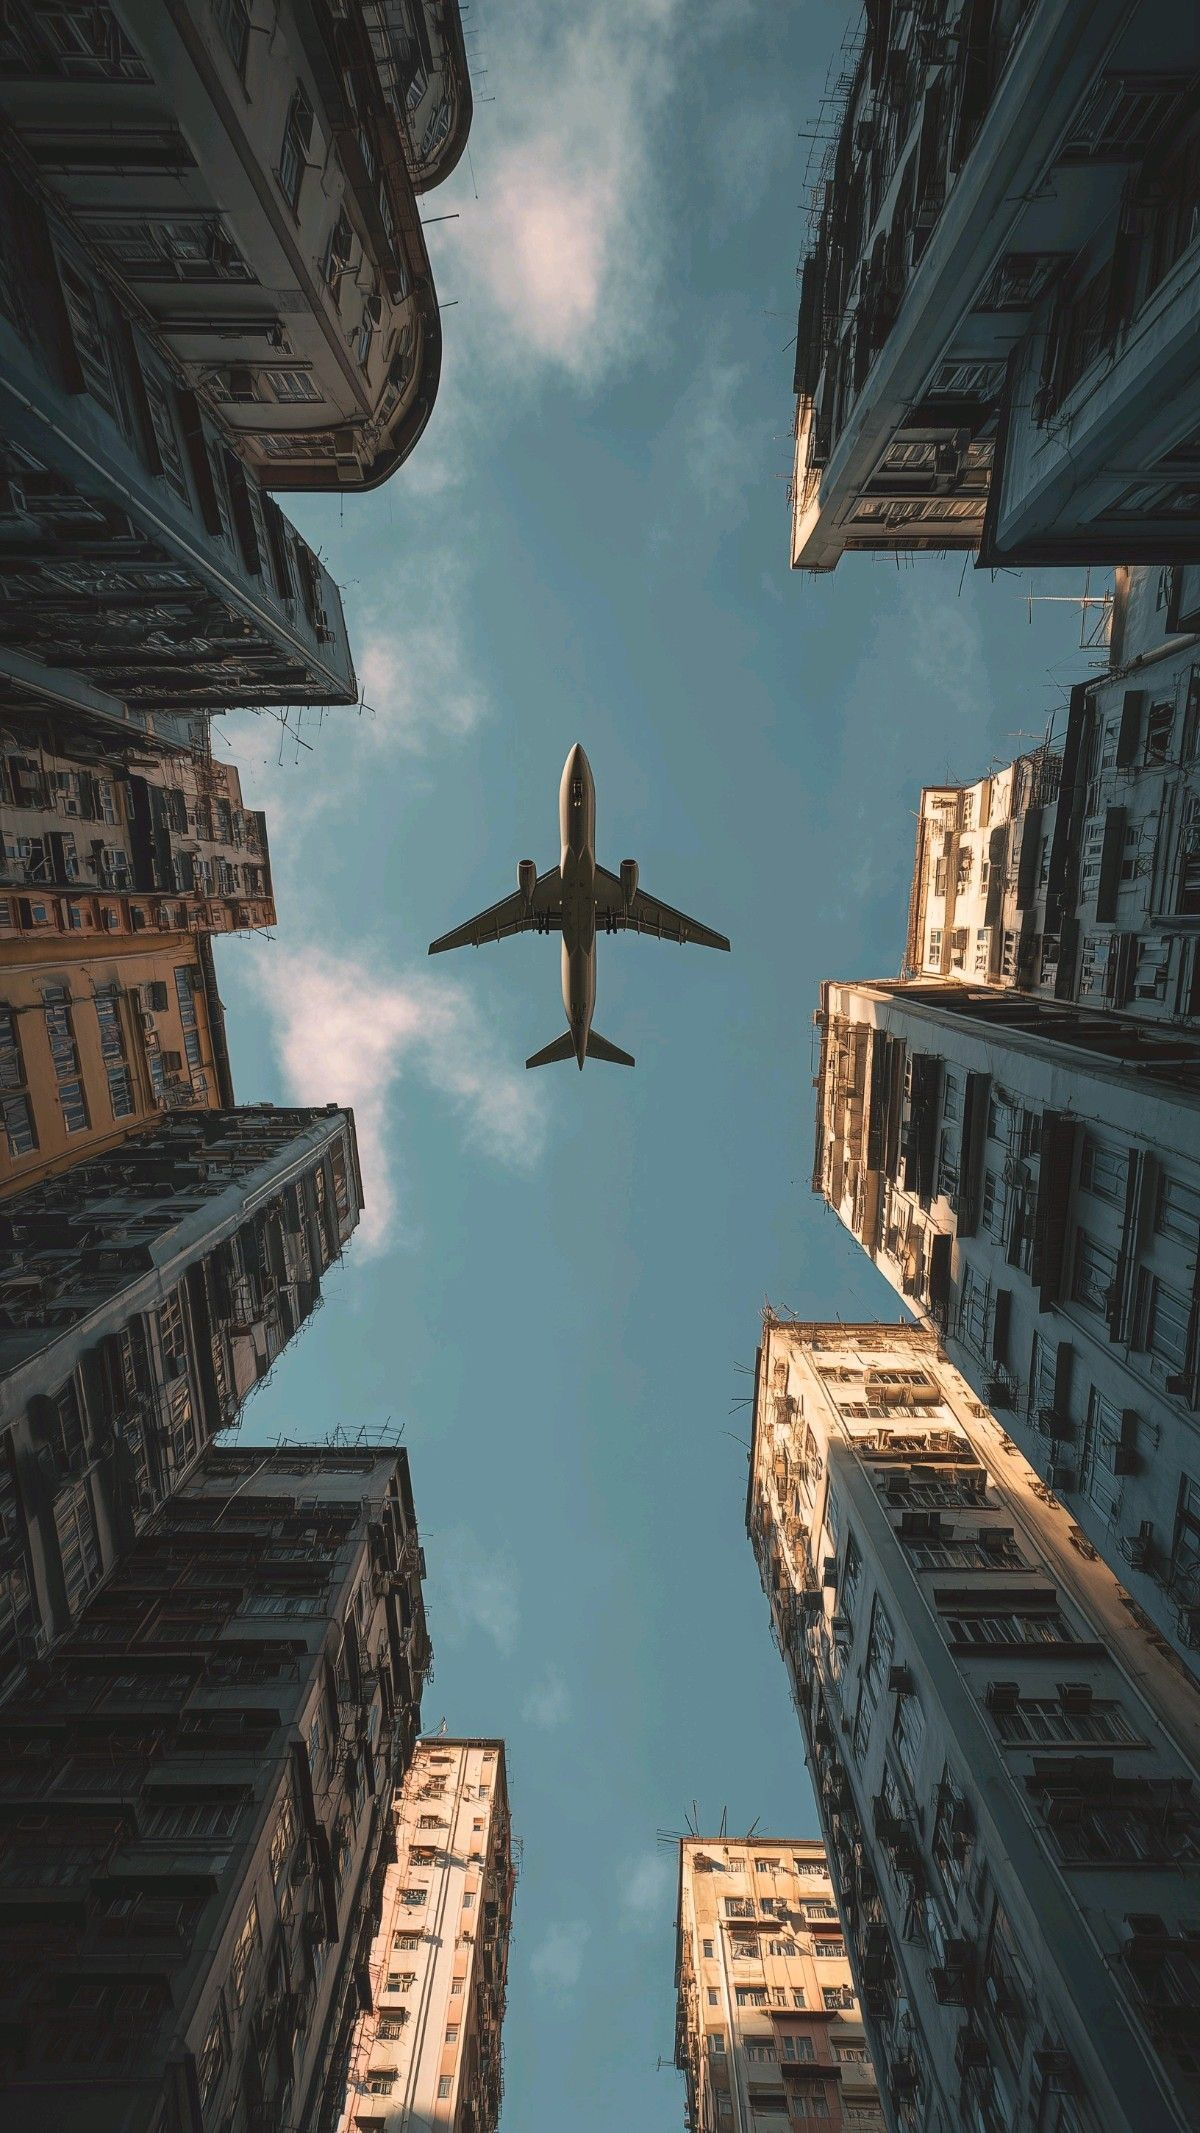
\includegraphics[width=1.1\linewidth]{plane.jpg}
\end{column}
\end{columns}
\end{frame}

% --- Slide 2 ---
\begin{frame}{Mục tiêu đề tài}
Ba mục tiêu cốt lõi:
\begin{enumerate}
  \item \textbf{Data Warehouse} theo Star Schema
  \begin{itemize}
    \item 1 bảng sự kiện (\texttt{fact\_flights}) + 4 bảng chiều.
    \item Pipeline ETL streaming theo chunk.
  \end{itemize}

  \item \textbf{Dashboard OLAP đa trang}
  \begin{itemize}
    \item 6 trang phân tích tương tác (Streamlit + Plotly).
    \item Hiện thực Slice, Dice, Roll-up, Drill-down.
  \end{itemize}

  \item \textbf{Mô hình dự báo delay}
  \begin{itemize}
    \item So sánh 5 thuật toán ML trên cùng pipeline.
    \item Đánh giá bằng 7 chỉ số, ưu tiên AUC-ROC.
  \end{itemize}
\end{enumerate}

\begin{block}{Đầu ra}
Dữ liệu thô $\rightarrow$ ETL $\rightarrow$ Kho dữ liệu $\rightarrow$ Dashboard + Mô hình dự báo.
\end{block}
\end{frame}

% --- Slide 3 ---
\begin{frame}{Nguồn dữ liệu}
Bộ dữ liệu công khai \textit{US Flight Delays 2015} (Kaggle):

\vspace{2mm}
\begin{table}
\centering
\small
\begin{tabular}{lrl}
\toprule
\textbf{Tệp} & \textbf{Số bản ghi} & \textbf{Nội dung} \\
\midrule
\texttt{flights.csv}  & 5.819.079 & 31 thuộc tính chuyến bay \\
\texttt{airlines.csv}  & 14 & Hãng hàng không nội địa \\
\texttt{airports.csv}  & 322 & Sân bay, vị trí, tọa độ \\
\bottomrule
\end{tabular}
\end{table}

\vspace{2mm}
\textbf{Phạm vi:} Chuyến bay nội địa Hoa Kỳ từ 01/01 đến 31/12/2015.
Không bao gồm chuyến bay quốc tế hoặc dữ liệu thời tiết thực tế.
\end{frame}

% --- Slide 4 ---
\begin{frame}{Thách thức chính}
\begin{columns}[T,onlytextwidth]
\begin{column}{0.45\textwidth}
\begin{enumerate}
  \item \textbf{Giá trị thiếu có cấu trúc}
  \begin{itemize}
    \item $\approx$76\% bản ghi thiếu chi tiết delay thành phần.
    \item Cột delay trống khi chuyến bị hủy hoặc chuyển hướng.
  \end{itemize}

  \item \textbf{Mất cân bằng lớp}
  \begin{itemize}
    \item $\approx$81\% đúng giờ vs. 19\% trễ.
    \item Imbalance ratio $\approx$ 4,23:1.
  \end{itemize}

  \item \textbf{Rò rỉ tương lai}
  \begin{itemize}
    \item \texttt{departure\_delay} chỉ biết \textit{sau} khi rời cổng.
    \item Phải loại để đảm bảo tính ``dự báo''.
  \end{itemize}
\end{enumerate}
\end{column}
\begin{column}{0.5\textwidth}
\centering
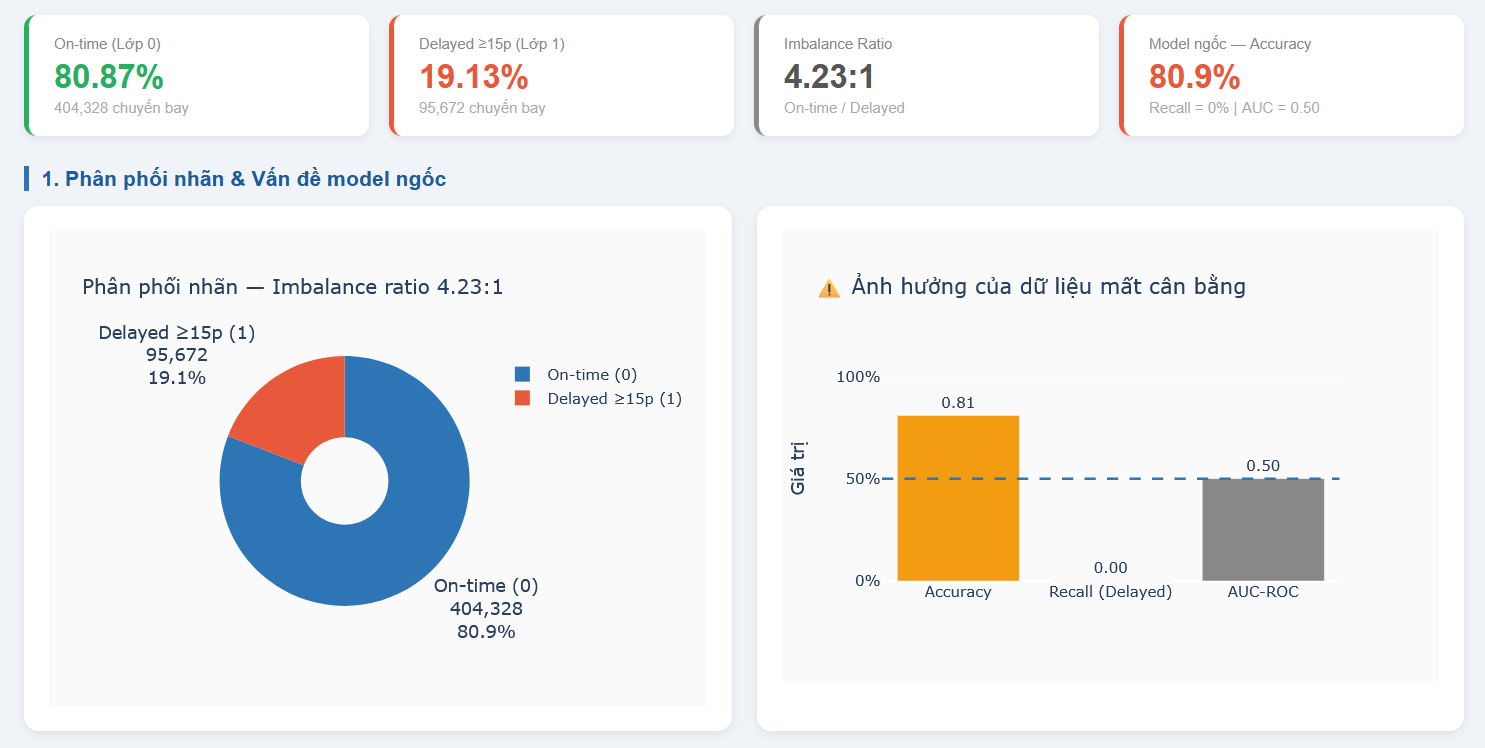
\includegraphics[width=\linewidth,height=0.65\textheight,keepaspectratio]{imbalance_analysis.png}
\end{column}
\end{columns}
\end{frame}


% ================= SECTION 2: CƠ SỞ LÝ THUYẾT =================
% ============================================================
% SECTION 2: CƠ SỞ LÝ THUYẾT
% ============================================================
\section{Cơ sở lý thuyết}

% --- Slide 5 ---
\begin{frame}{Data Warehouse và Star Schema}
\begin{columns}[T,onlytextwidth]
\begin{column}{0.52\textwidth}
\textbf{Data Warehouse}
\begin{itemize}
  \item Hướng chủ đề (\textit{subject-oriented}).
  \item Tích hợp, không biến động, biến thiên theo thời gian.
  \item Tối ưu cho truy vấn phân tích (khác OLTP).
\end{itemize}

\vspace{2mm}
\textbf{Star Schema} (Ralph Kimball)
\begin{itemize}
  \item \textbf{Fact table}: đo lường định lượng (delay, distance, cờ trễ).
  \item \textbf{Dimension tables}: ngữ cảnh (hãng, sân bay, ngày, nguyên nhân).
  \item Ít JOIN, truy vấn nhanh, dễ hiểu.
\end{itemize}
\end{column}
\begin{column}{0.48\textwidth}
\centering
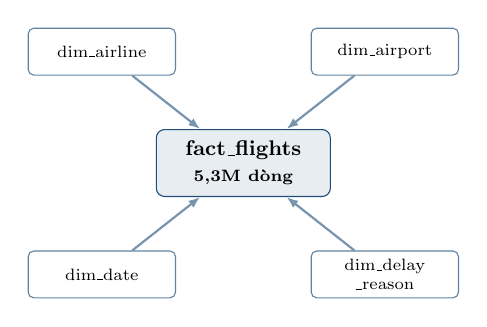
\begin{tikzpicture}[
  scale=0.85, transform shape,
  fact/.style={rectangle, draw=BKTemplate, fill=BKTemplate!10,
    minimum width=2.6cm, minimum height=1cm, align=center,
    font=\small\bfseries, rounded corners=3pt},
  dim/.style={rectangle, draw=BKTemplate!70, fill=white,
    minimum width=2.2cm, minimum height=0.7cm, align=center,
    font=\scriptsize, rounded corners=2pt},
  arr/.style={-{Latex[length=1.5mm]}, thick, BKTemplate!60}
]
\node[fact] (f) {fact\_flights\\{\scriptsize 5,3M dòng}};
\node[dim, above left=8mm and -3mm of f]  (d1) {dim\_airline};
\node[dim, above right=8mm and -3mm of f] (d2) {dim\_airport};
\node[dim, below left=8mm and -3mm of f]  (d3) {dim\_date};
\node[dim, below right=8mm and -3mm of f] (d4) {dim\_delay\\\_reason};
\draw[arr] (d1) -- (f);
\draw[arr] (d2) -- (f);
\draw[arr] (d3) -- (f);
\draw[arr] (d4) -- (f);
\end{tikzpicture}
\end{column}
\end{columns}
\end{frame}

% --- Slide 6 ---
\begin{frame}{Phân tích OLAP đa chiều}
\textbf{OLAP} (Online Analytical Processing): phân tích dữ liệu đa chiều, tương tác.

\vspace{2mm}
\begin{columns}[T,onlytextwidth]
\begin{column}{0.48\textwidth}
\begin{block}{5 phép OLAP cơ bản}
\begin{description}[\textbf{Drill-down}]
  \item[\textbf{Roll-up}] Tổng hợp lên: tháng $\to$ quý $\to$ năm.
  \item[\textbf{Drill-down}] Phân rã: hãng $\to$ từng chuyến.
  \item[\textbf{Slice}] Cắt 1 chiều: chỉ xem tháng 12.
  \item[\textbf{Dice}] Lọc nhiều chiều cùng lúc.
  \item[\textbf{Pivot}] Xoay trục nhìn Data Cube.
\end{description}
\end{block}
\end{column}
\begin{column}{0.48\textwidth}
\begin{block}{Ánh xạ trong đề tài}
\begin{itemize}
  \item Bộ lọc sidebar = \textbf{Slice / Dice}.
  \item Chuyển tháng $\leftrightarrow$ quý = \textbf{Roll-up / Drill-down}.
  \item Xem theo hãng vs. theo sân bay = \textbf{Pivot}.
\end{itemize}
\end{block}
\end{column}
\end{columns}
\end{frame}

% --- Slide 7 ---
\begin{frame}{Tiền xử lý dữ liệu}
4 giai đoạn (áp dụng cụ thể cho dữ liệu hàng không):

\vspace{2mm}
\begin{columns}[T,onlytextwidth]
\begin{column}{0.5\textwidth}
\textbf{1. Data Cleaning}
\begin{itemize}
  \item \textbf{Missing}: $\sim$76\% delay thành phần thiếu $\to$ \texttt{fillna(0)}.
  \item \textbf{Outliers}: delay âm = đến sớm (bình thường); delay cực lớn = thật.
  \item Nhãn nhị phân ``trung hòa'' giá trị cực đoan.
\end{itemize}

\vspace{1mm}
\textbf{2. Data Integration}
\begin{itemize}
  \item 3 CSV $\to$ lookup join qua surrogate key.
\end{itemize}
\end{column}
\begin{column}{0.5\textwidth}
\textbf{3. Data Transformation}
\begin{itemize}
  \item Z-score cho LR, MLP.
  \item Feature construction: \texttt{dep\_hour}, \texttt{is\_weekend}, \texttt{quarter}.
  \item Label Encoding cho hãng, bang.
\end{itemize}

\vspace{1mm}
\textbf{4. Data Reduction}
\begin{itemize}
  \item 31 cột $\to$ \textbf{10 đặc trưng} biết trước khi cất cánh.
  \item Class weights thay vì over/under-sampling.
\end{itemize}
\end{column}
\end{columns}
\end{frame}

% --- Slide 8 ---
\begin{frame}{Năm thuật toán khai phá dữ liệu}
\small
\begin{table}
\centering
\scriptsize
\begin{tabular}{clll}
\toprule
\textbf{\#} & \textbf{Thuật toán} & \textbf{Trường phái} & \textbf{Đặc điểm chính} \\
\midrule
1 & Logistic Regression & Tuyến tính & Nhanh, giải thích được, baseline \\
2 & Random Forest & Bagging & $T$ cây song song, robust, feature importance \\
3 & Neural Network (MLP) & Deep Learning & Nhiều lớp ẩn phi tuyến, ReLU + Adam \\
4 & XGBoost & Boosting & Cây tuần tự sửa residual, regularization L1/L2 \\
5 & LightGBM & Boosting & Leaf-wise + histogram splitting, nhanh hơn XGBoost \\
\bottomrule
\end{tabular}
\end{table}

\vspace{2mm}
\begin{block}{Gradient Boosting vs. Random Forest}
\begin{itemize}
  \item RF: cây xây \textbf{độc lập} $\to$ majority vote.
  \item GBDT: cây xây \textbf{tuần tự}, mỗi cây sửa lỗi cây trước:
        $F_m(\mathbf{x}) = F_{m-1}(\mathbf{x}) + \eta \cdot h_m(\mathbf{x})$.
\end{itemize}
\end{block}
\end{frame}

% --- Slide 9 ---
\begin{frame}{Chỉ số đánh giá}
Với dữ liệu mất cân bằng (81\% / 19\%), chỉ số đánh giá rất quan trọng:

\vspace{2mm}
\small
\begin{table}
\centering
\begin{tabular}{lp{7.8cm}}
\toprule
\textbf{Chỉ số} & \textbf{Ý nghĩa} \\
\midrule
\textbf{AUC-ROC} & Khả năng phân biệt 2 lớp ở mọi ngưỡng (chỉ số \textbf{chính}) \\
Accuracy & Tỷ lệ đúng tổng thể --- \textcolor{red}{gây hiểu nhầm khi lệch lớp} \\
F1-score & Trung bình hài hòa Precision--Recall \\
Avg. Precision & Diện tích dưới Precision-Recall --- nhạy hơn AUC khi lớp dương nhỏ \\
Log Loss & Chất lượng xác suất dự đoán (thấp hơn = tốt hơn) \\
Brier Score & Bình phương sai lệch xác suất--nhãn (thấp hơn = tốt hơn) \\
TG huấn luyện & Chi phí tính toán thực tế \\
\bottomrule
\end{tabular}
\end{table}

\vspace{2mm}
Mô hình luôn đoán ``đúng giờ'' đạt Accuracy $\approx$81\% nhưng AUC = 0,50
$\to$ \textbf{Accuracy đơn thuần gây hiểu nhầm}.
\end{frame}


% ================= SECTION 3: THIẾT KẾ HỆ THỐNG =================
% ============================================================
% SECTION 3: THIẾT KẾ HỆ THỐNG
% ============================================================
\section{Thiết kế hệ thống}

% --- Slide 10 ---
\begin{frame}{Kiến trúc tổng thể}
\centering
\resizebox{0.78\linewidth}{!}{%
\begin{tikzpicture}[
  node distance=7mm,
  box/.style={
    rectangle, rounded corners=4pt, draw=BKTemplate, fill=white,
    line width=0.9pt, align=center, inner sep=6pt,
    minimum height=1.15cm, text width=3.2cm
  },
  widebox/.style={
    rectangle, rounded corners=4pt, draw=BKTemplate, fill=white,
    line width=0.9pt, align=center, inner sep=7pt,
    minimum height=1.15cm, text width=8cm
  },
  arr/.style={-{Latex[length=2mm]}, thick, BKTemplate}
]
\node[widebox] (src) {\textbf{Nguồn dữ liệu thô}\\\scriptsize flights.csv, airlines.csv, airports.csv};
\node[widebox, below=of src] (etl) {\textbf{Tầng ETL}\\\scriptsize extract $\rightarrow$ transform $\rightarrow$ load theo chunk};
\node[widebox, below=of etl] (dw) {\textbf{Data Warehouse SQLite}\\\scriptsize Star Schema: 1 fact + 4 dimension tables};
\node[box, below left=12mm and 10mm of dw] (dash) {\textbf{Dashboard OLAP}\\\scriptsize 6 trang phân tích tương tác};
\node[box, below right=12mm and 10mm of dw] (mine) {\textbf{Data Mining}\\\scriptsize 500K mẫu, 5 models};

\draw[arr] (src) -- (etl);
\draw[arr] (etl) -- (dw);

\coordinate (fork) at ([yshift=-8mm]dw.south);
\draw[thick, BKTemplate] (dw.south) -- (fork);
\draw[arr] (fork) -| (dash.north);
\draw[arr] (fork) -| (mine.north);
\end{tikzpicture}%
}

\vspace{1mm}
\small Luồng chính \textbf{một chiều}: thô $\rightarrow$ ETL $\rightarrow$ kho.
Dashboard và Mining đều \textbf{chỉ đọc} từ kho.
\end{frame}

% --- Slide 11 ---
\begin{frame}{Nguyên tắc luồng dữ liệu}
\begin{enumerate}
  \item \textbf{Luồng chính một chiều}\\
        Nguồn thô $\rightarrow$ ETL $\rightarrow$ Kho.
        Có thể tái tạo bất kỳ lúc nào bằng cách chạy lại ETL.

  \item \textbf{Hai lớp tiêu thụ chỉ đọc}\\
        Dashboard và Mining đều chỉ \textbf{đọc} từ kho, không ghi ngược.
        Giữ schema ổn định, tránh xung đột dữ liệu.

  \item \textbf{Chia sẻ kết quả giữa 2 lớp}\\
        Dashboard gọi mô hình từ lớp Mining (hiển thị xác suất trễ)
        --- kết nối ở mức ứng dụng, không thay đổi kho.
\end{enumerate}

\vspace{3mm}
\begin{block}{Lợi ích}
Mỗi lớp phát triển và kiểm thử \textbf{độc lập}:
thay đổi logic dashboard $\not\Rightarrow$ sửa ETL;
thêm thuật toán mới $\not\Rightarrow$ sửa schema kho.
\end{block}
\end{frame}

% --- Slide 12 ---
\begin{frame}{Star Schema: Mô hình dữ liệu}
\begin{columns}[T,onlytextwidth]
\begin{column}{0.55\textwidth}
\textbf{Bảng sự kiện} \texttt{fact\_flights}
\begin{itemize}
  \item $\approx$ 5,3M bản ghi sau ETL.
  \item FK tới 4 bảng chiều.
  \item Đo lường: delay, distance, elapsed time,
        cờ hủy/chuyển hướng/trễ $\geq$15p.
\end{itemize}

\vspace{2mm}
\textbf{4 bảng chiều}
\begin{itemize}
  \item \texttt{dim\_airline}: 14 hãng.
  \item \texttt{dim\_airport}: 322 sân bay (IATA, bang, tọa độ).
  \item \texttt{dim\_date}: 365 ngày (năm$\to$quý$\to$tháng$\to$tuần$\to$thứ).
  \item \texttt{dim\_delay\_reason}: 6 loại nguyên nhân.
\end{itemize}
\end{column}
\begin{column}{0.45\textwidth}
\small
\begin{tabular}{l r}
\toprule
\textbf{Bảng} & \textbf{Số dòng} \\
\midrule
\texttt{fact\_flights}     & 5{,}332{,}914 \\
\texttt{dim\_airline}      & 14 \\
\texttt{dim\_airport}      & 322 \\
\texttt{dim\_date}         & 365 \\
\texttt{dim\_delay\_reason}& 6 \\
\bottomrule
\end{tabular}

\vspace{4mm}
\begin{block}{Ưu điểm}
\begin{itemize}
  \item Truy vấn đơn giản, ít JOIN.
  \item 6 chỉ mục OLAP.
  \item Đủ nhẹ cho SQLite.
\end{itemize}
\end{block}
\end{column}
\end{columns}
\end{frame}

% --- Slide 13 ---
\begin{frame}{Pipeline ETL}
\begin{columns}[T,onlytextwidth]
\begin{column}{0.55\textwidth}
\textbf{4 bước tuần tự:}
\begin{enumerate}
  \item \textbf{Đọc dimension nhỏ}\\
        \texttt{airlines.csv}, \texttt{airports.csv} vào RAM;
        quét \texttt{flights.csv} 1 lần $\to$ \texttt{dim\_date}.
  \item \textbf{Khởi tạo schema}\\
        \texttt{schema.sql} + PRAGMA WAL.
  \item \textbf{Nạp dimension + lookup maps}\\
        Dictionary ánh xạ surrogate key.
  \item \textbf{Streaming fact\_flights}\\
        Chunk 100K dòng $\to$ transform $\to$ INSERT batch $\to$ giải phóng RAM.
\end{enumerate}
\end{column}
\begin{column}{0.45\textwidth}
\textbf{Tối ưu:}
\begin{itemize}
  \item \texttt{float32/int8/int16} thay \texttt{float64} $\to$ RAM $\approx$120 MB/chunk.
  \item \texttt{numpy.select} vectorized cho phân loại delay.
  \item Hoàn thành trong \textbf{3--8 phút}.
\end{itemize}

\vspace{2mm}
\textbf{Xử lý missing:}
\begin{itemize}
  \item Cột delay: \texttt{fillna(0.0)}.
  \item Thiếu FK: \texttt{dropna} loại dòng.
  \item Kết quả: giữ $\approx$91,65\% bản ghi.
\end{itemize}
\end{column}
\end{columns}
\end{frame}


% ================= SECTION 4: DASHBOARD =================
% ============================================================
% SECTION 4: DASHBOARD
% ============================================================
\section{Dashboard OLAP}

% --- Slide 14 ---
\begin{frame}{Tổng quan Dashboard}
\begin{itemize}
  \item Xây dựng bằng \textbf{Streamlit} + \textbf{Plotly}, kết nối trực tiếp \texttt{airline\_dw.db}.
  \item \textbf{6 trang} điều hướng qua sidebar:
\end{itemize}

\vspace{2mm}
\small
\begin{table}
\centering
\begin{tabular}{clp{6.5cm}}
\toprule
\textbf{\#} & \textbf{Trang} & \textbf{Chức năng} \\
\midrule
1 & Tổng quan & KPI toàn ngành, cơ cấu chuyến, xu hướng delay \\
2 & Tuyến đường & Top tuyến theo hãng, lọc địa lý bang/sân bay \\
3 & Thời gian & Mùa vụ, thứ trong tuần, khung giờ bay \\
4 & Nguyên nhân & Cơ cấu delay, đóng góp tổng phút trễ \\
5 & Dự báo & Form nhập $\to$ xác suất delay thời gian thực \\
6 & Database Explorer & Schema, thống kê bảng, SQL tùy chỉnh \\
\bottomrule
\end{tabular}
\end{table}

\vspace{2mm}
Bộ lọc chung: \textbf{tháng/quý} + \textbf{hãng IATA} --- áp dụng cho 4 trang phân tích.
\end{frame}

% --- Slide 15 ---
\begin{frame}{Trang Tổng quan}
\begin{columns}[T,onlytextwidth]
\begin{column}{0.48\textwidth}
\textbf{5 KPI} (phản ứng theo bộ lọc):
\begin{itemize}
  \item Tổng chuyến bay: \textbf{5.332.914}
  \item OTP toàn ngành: \textbf{81,19\%}
  \item Tỉ lệ delay $\geq$15p: \textbf{18,81\%}
  \item Tỉ lệ hủy chuyến: \textbf{1,64\%}
  \item Delay trung bình: \textbf{4,8 phút}
\end{itemize}

\vspace{1mm}
\textbf{Biểu đồ:}
\begin{itemize}
  \item Cơ cấu chuyến bay theo tháng (cột chồng).
  \item Top 5 hãng OTP / Top 5 sân bay delay cao.
  \item Xu hướng delay \& hủy theo tháng.
\end{itemize}
\end{column}
\begin{column}{0.48\textwidth}
\centering
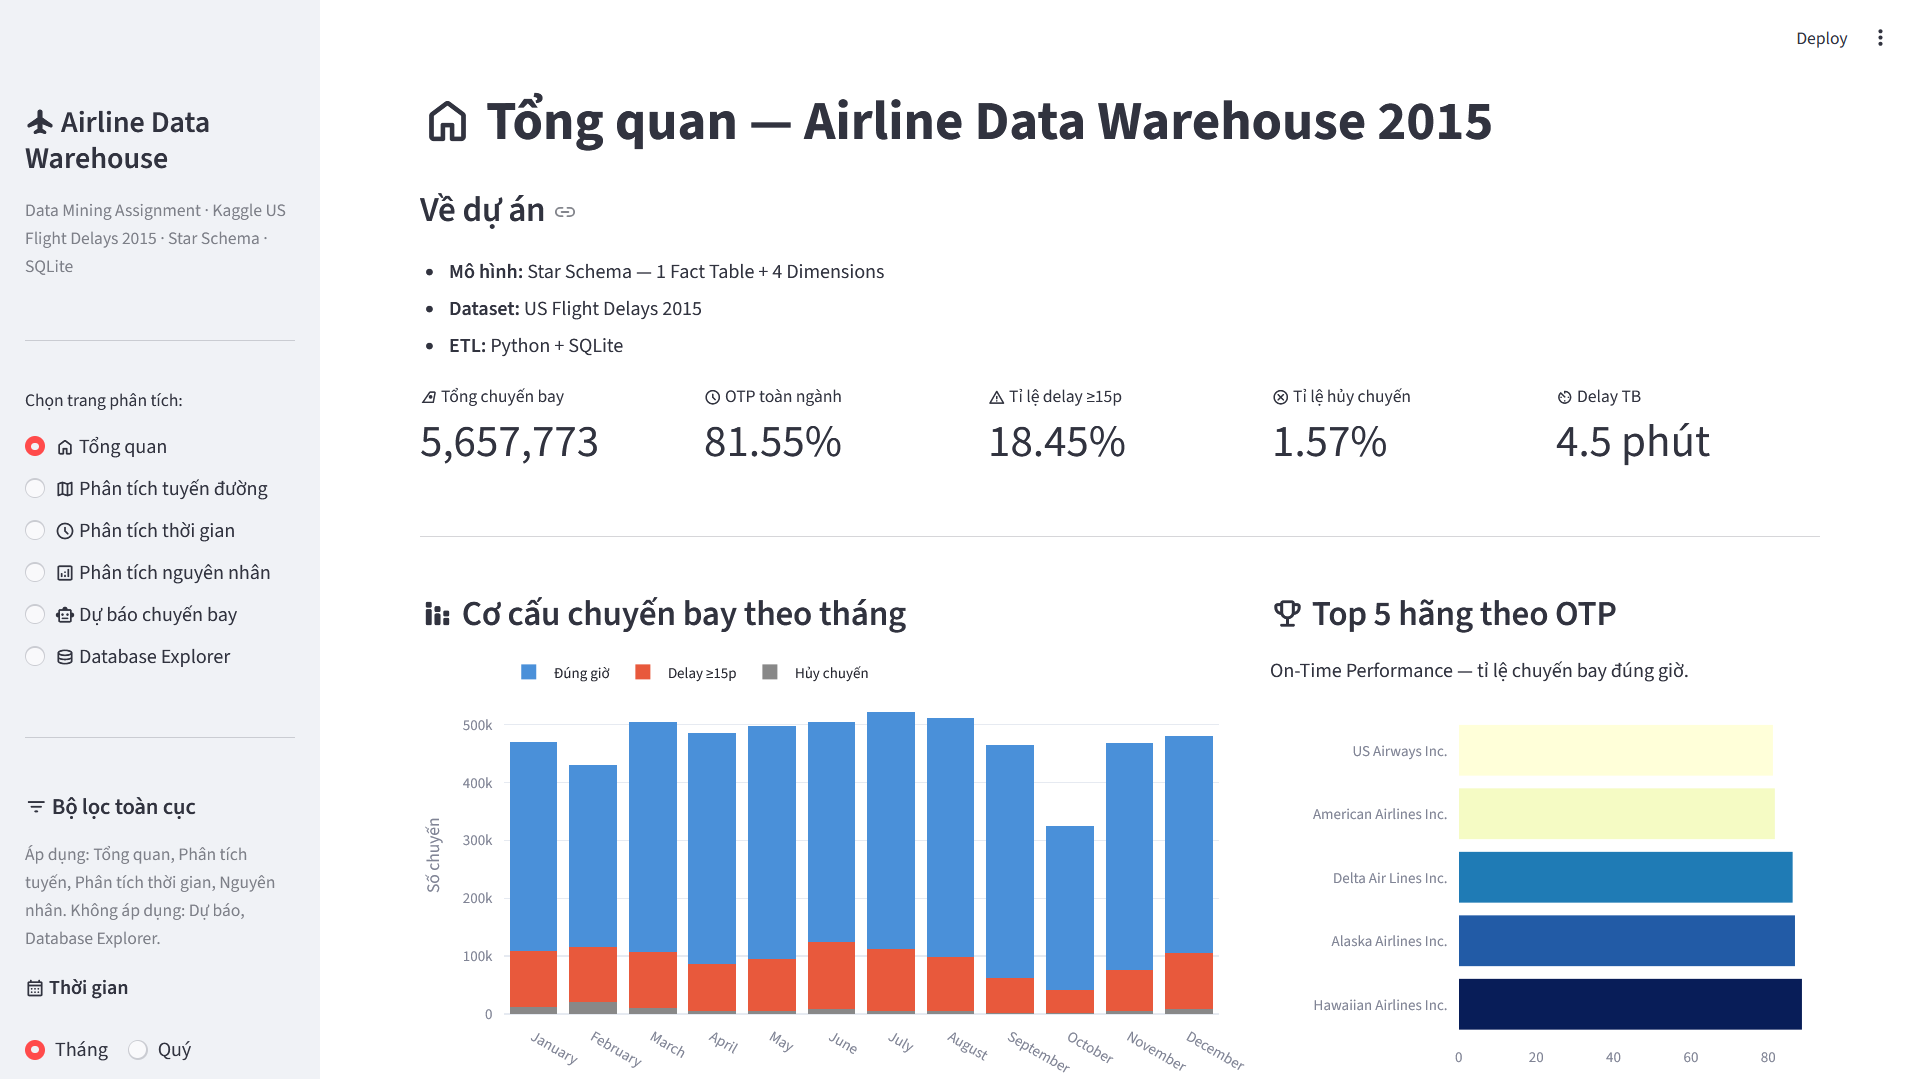
\includegraphics[width=\linewidth,height=0.7\textheight,keepaspectratio]{overview.png}
\end{column}
\end{columns}
\end{frame}

% --- Slide 16 ---
\begin{frame}{Trang Phân tích tuyến đường}
\begin{columns}[T,onlytextwidth]
\begin{column}{0.48\textwidth}
\begin{itemize}
  \item Top tuyến bay (cặp sân bay đi $\to$ đến) theo từng hãng.
  \item Bộ lọc địa lý: \textbf{bang xuất phát / bang đích},
        sau đó lọc tiếp theo sân bay cụ thể.
  \item Mỗi hãng sinh khối biểu đồ riêng,
        số tuyến và ngưỡng tối thiểu điều chỉnh được.
\end{itemize}
\end{column}
\begin{column}{0.48\textwidth}
\centering
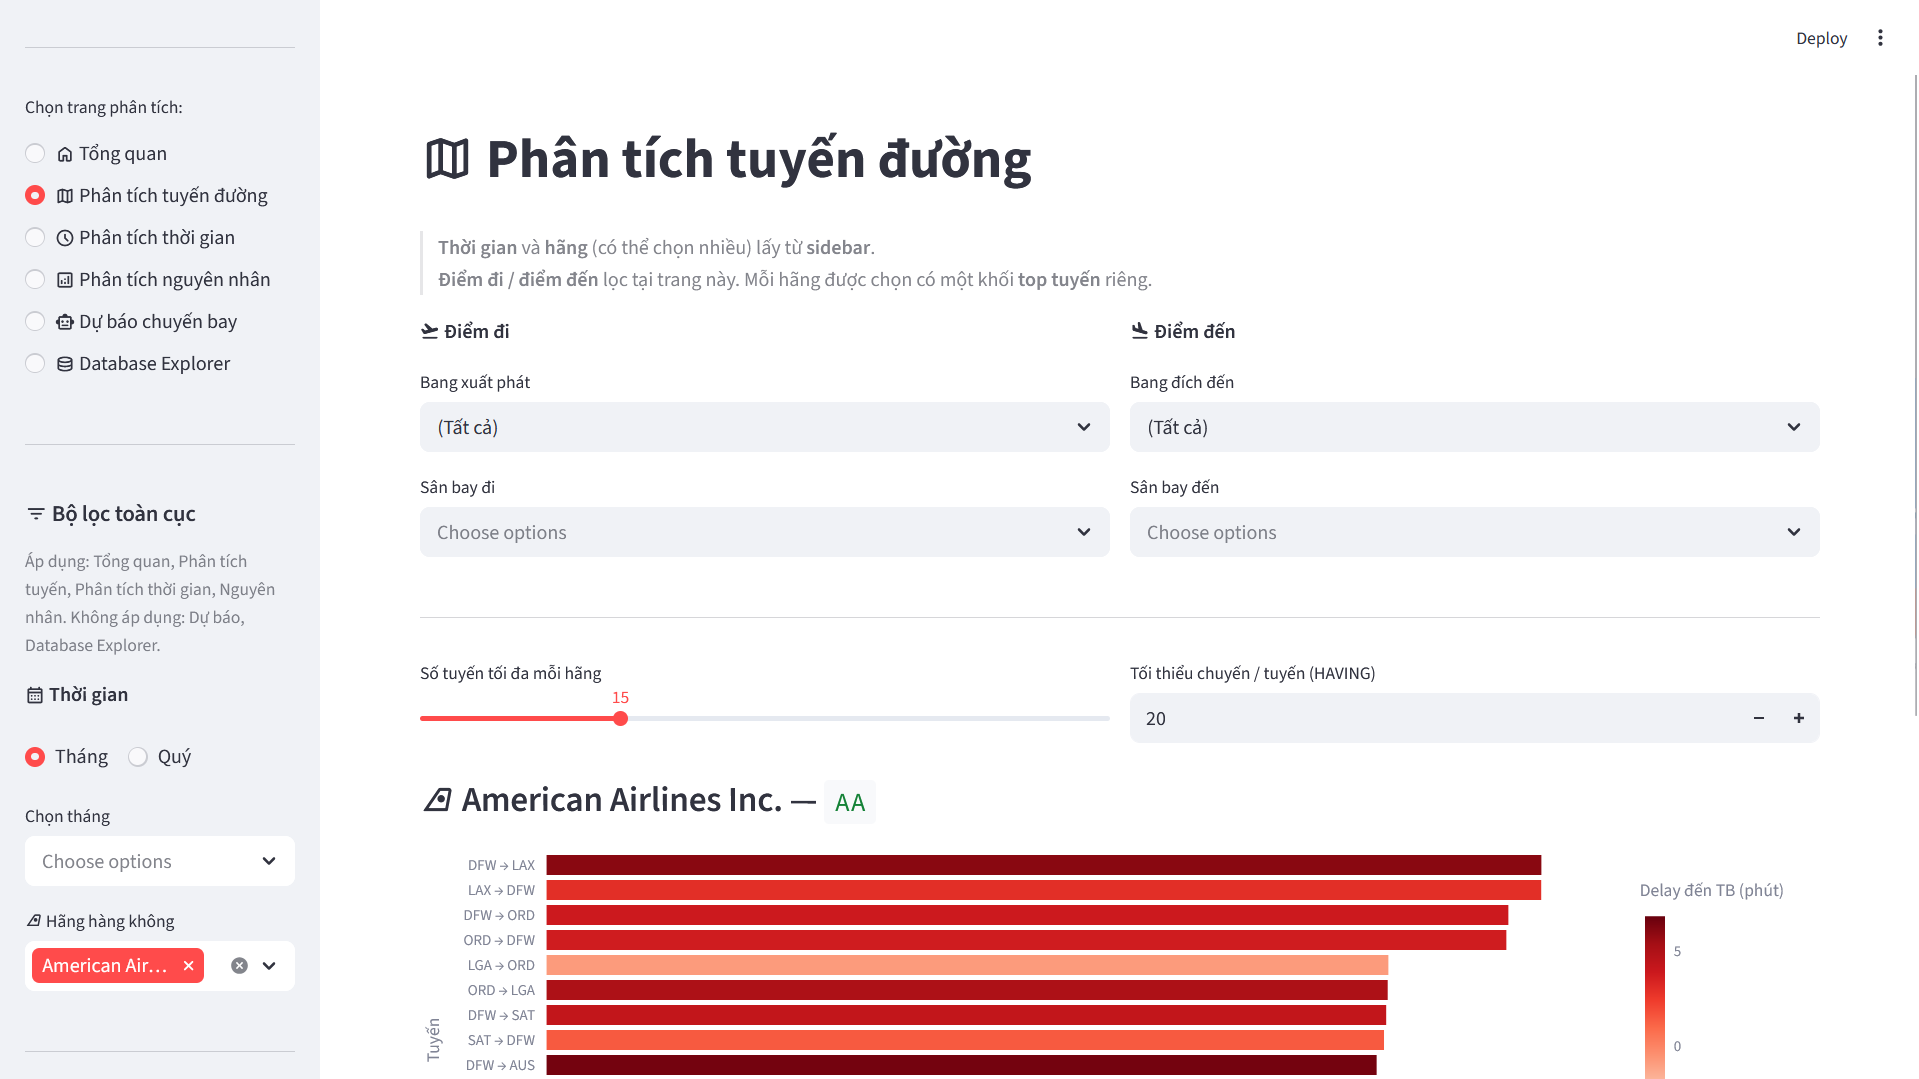
\includegraphics[width=\linewidth,height=0.7\textheight,keepaspectratio]{routes.png}
\end{column}
\end{columns}
\end{frame}

% --- Slide 17 ---
\begin{frame}{Trang Phân tích thời gian}
\begin{columns}[T,onlytextwidth]
\begin{column}{0.48\textwidth}
\begin{itemize}
  \item \textbf{Theo tháng}: heatmap số chuyến $\times$ nguyên nhân;
        delay TB tô màu theo mùa.
  \item \textbf{Theo quý}: cột delay TB Q1--Q4.
  \item \textbf{Theo thứ}: phút TB và tỷ lệ $\geq$15\%.
  \item So sánh ngày thường vs. cuối tuần:
        \textbf{5,4 phút} vs. \textbf{3,4 phút}.
  \item Delay theo \textbf{4 khung giờ} cất cánh.
\end{itemize}
\end{column}
\begin{column}{0.48\textwidth}
\centering
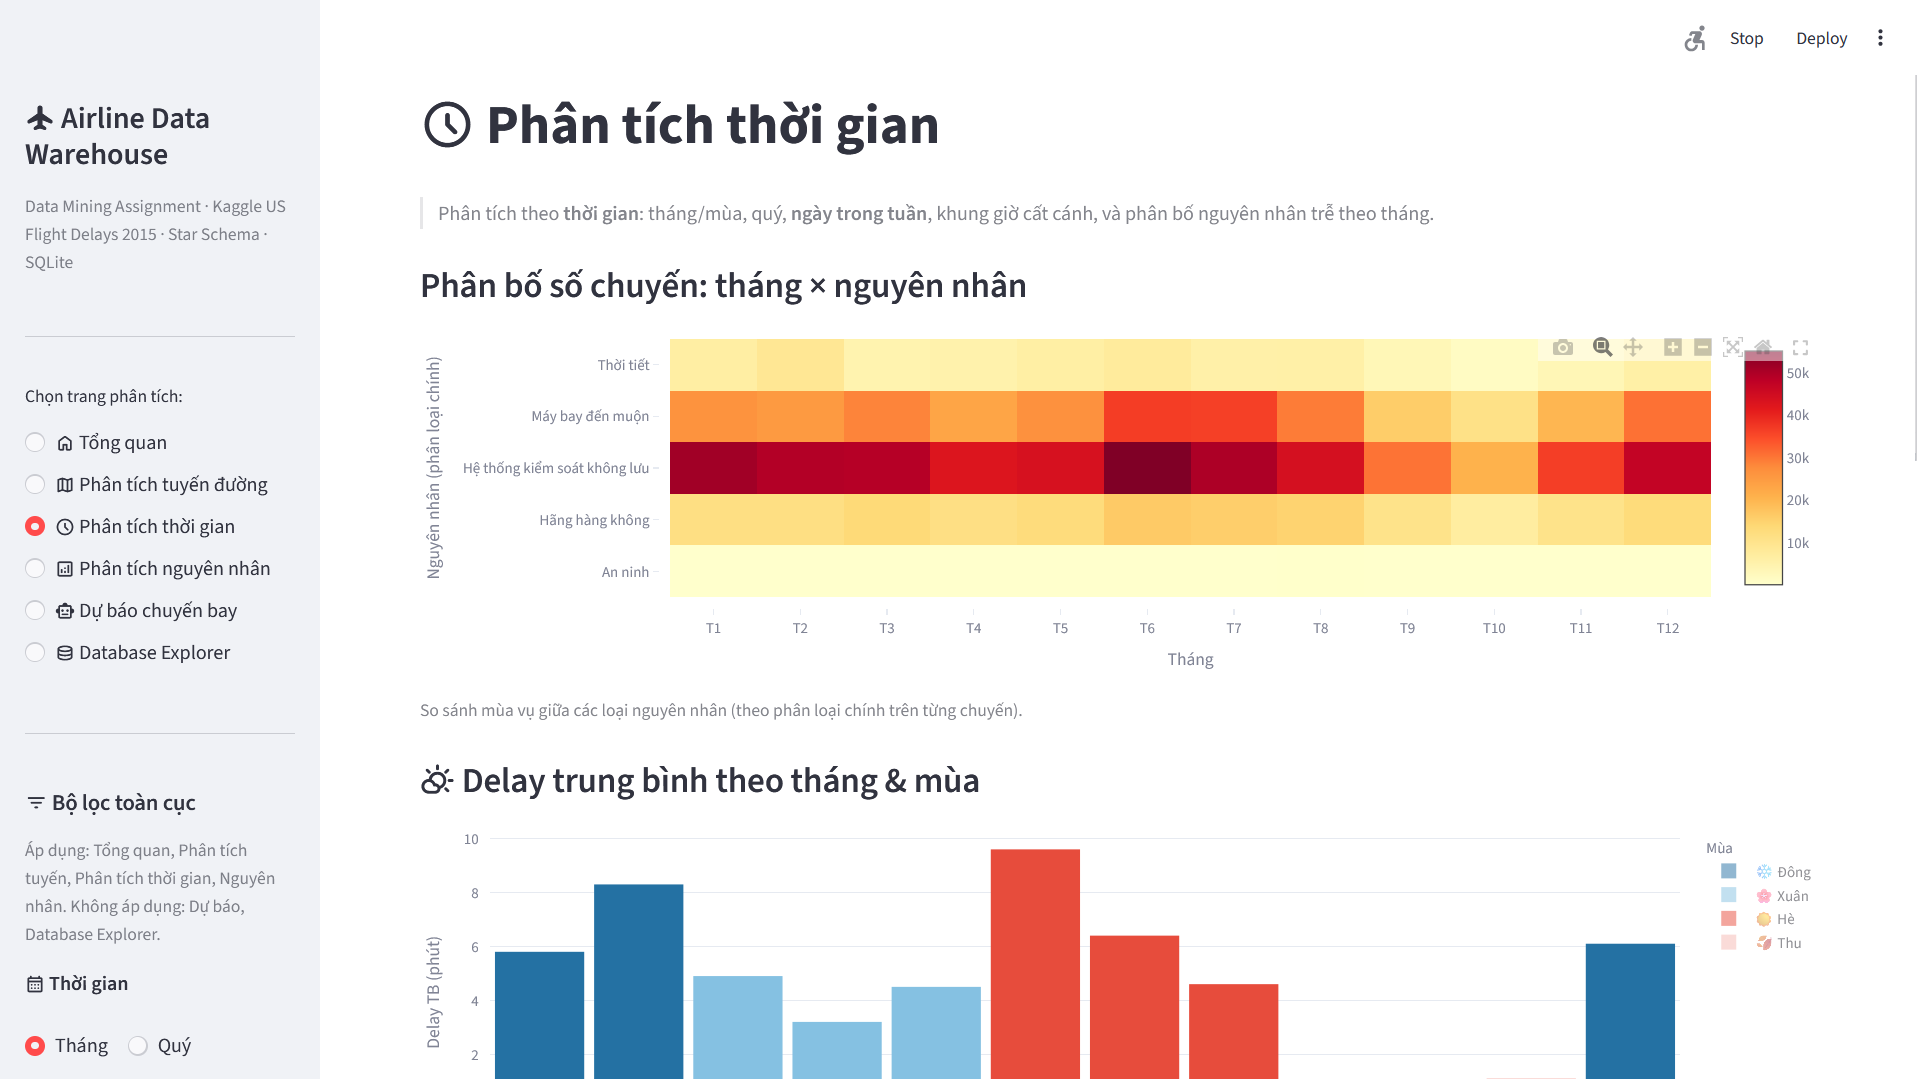
\includegraphics[width=\linewidth,height=0.7\textheight,keepaspectratio]{time.png}
\end{column}
\end{columns}
\end{frame}

% --- Slide 18 ---
\begin{frame}{Trang Phân tích nguyên nhân}
\begin{columns}[T,onlytextwidth]
\begin{column}{0.48\textwidth}
\begin{itemize}
  \item Pie cơ cấu số chuyến theo nguyên nhân.
  \item Cột ngang delay TB theo từng loại.
  \item Bảng tóm tắt: số chuyến, \%, delay TB, tổng phút trễ.
  \item Biểu đồ \textbf{đóng góp tổng phút trễ} --- nguyên nhân nào
        chiếm thời gian chờ lớn nhất?
\end{itemize}

\vspace{2mm}
\textbf{5 nguyên nhân:}\\
NAS, Late Aircraft, Carrier, Weather, Security.
\end{column}
\begin{column}{0.48\textwidth}
\centering
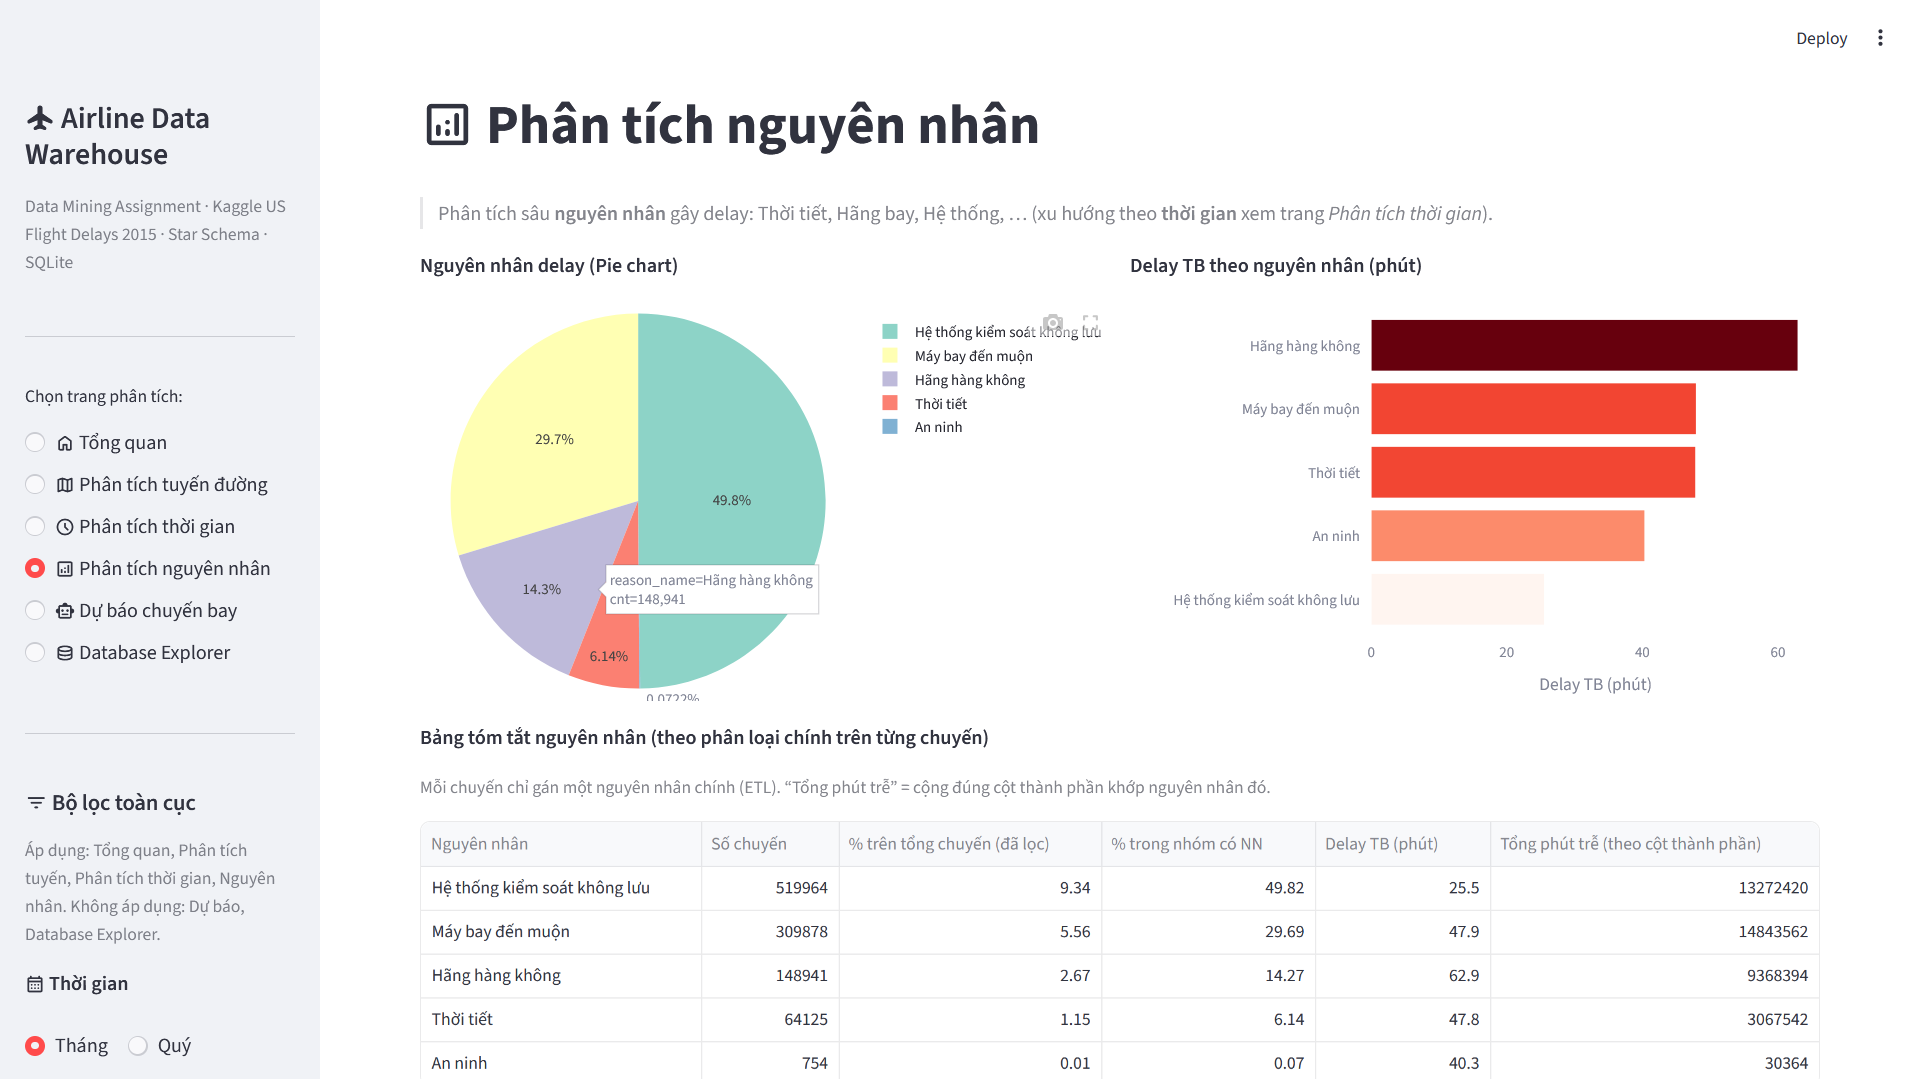
\includegraphics[width=\linewidth,height=0.7\textheight,keepaspectratio]{reason.png}
\end{column}
\end{columns}
\end{frame}

% --- Slide 19 ---
\begin{frame}{Trang Dự báo \& Database Explorer}
\begin{columns}[T,onlytextwidth]
\begin{column}{0.48\textwidth}
\centering
\textbf{Dự báo chuyến bay}\\[2mm]
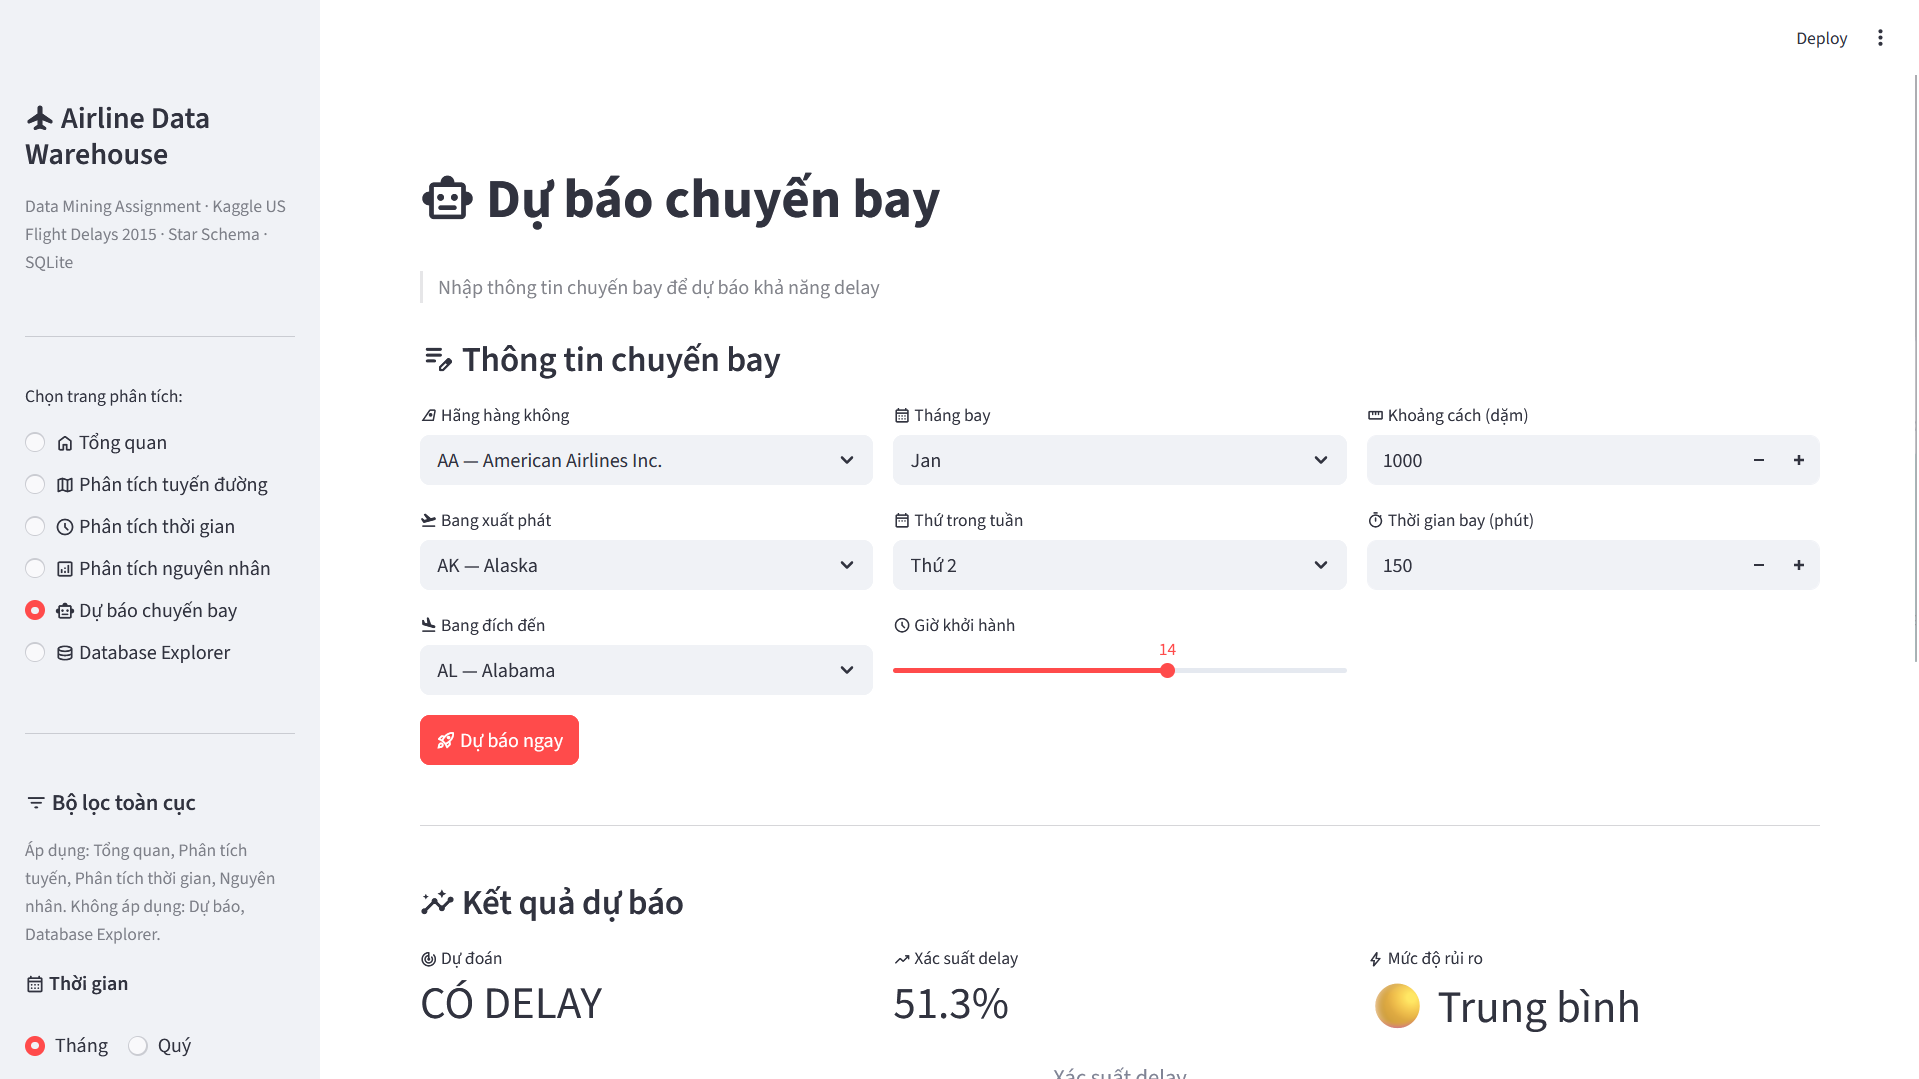
\includegraphics[width=\linewidth,height=0.48\textheight,keepaspectratio]{predict.png}\\
\scriptsize Form: hãng, bang đi/đến, tháng, thứ, giờ, distance, elapsed time
$\to$ nhãn + xác suất + gauge Plotly.
\end{column}
\begin{column}{0.48\textwidth}
\centering
\textbf{Database Explorer}\\[2mm]
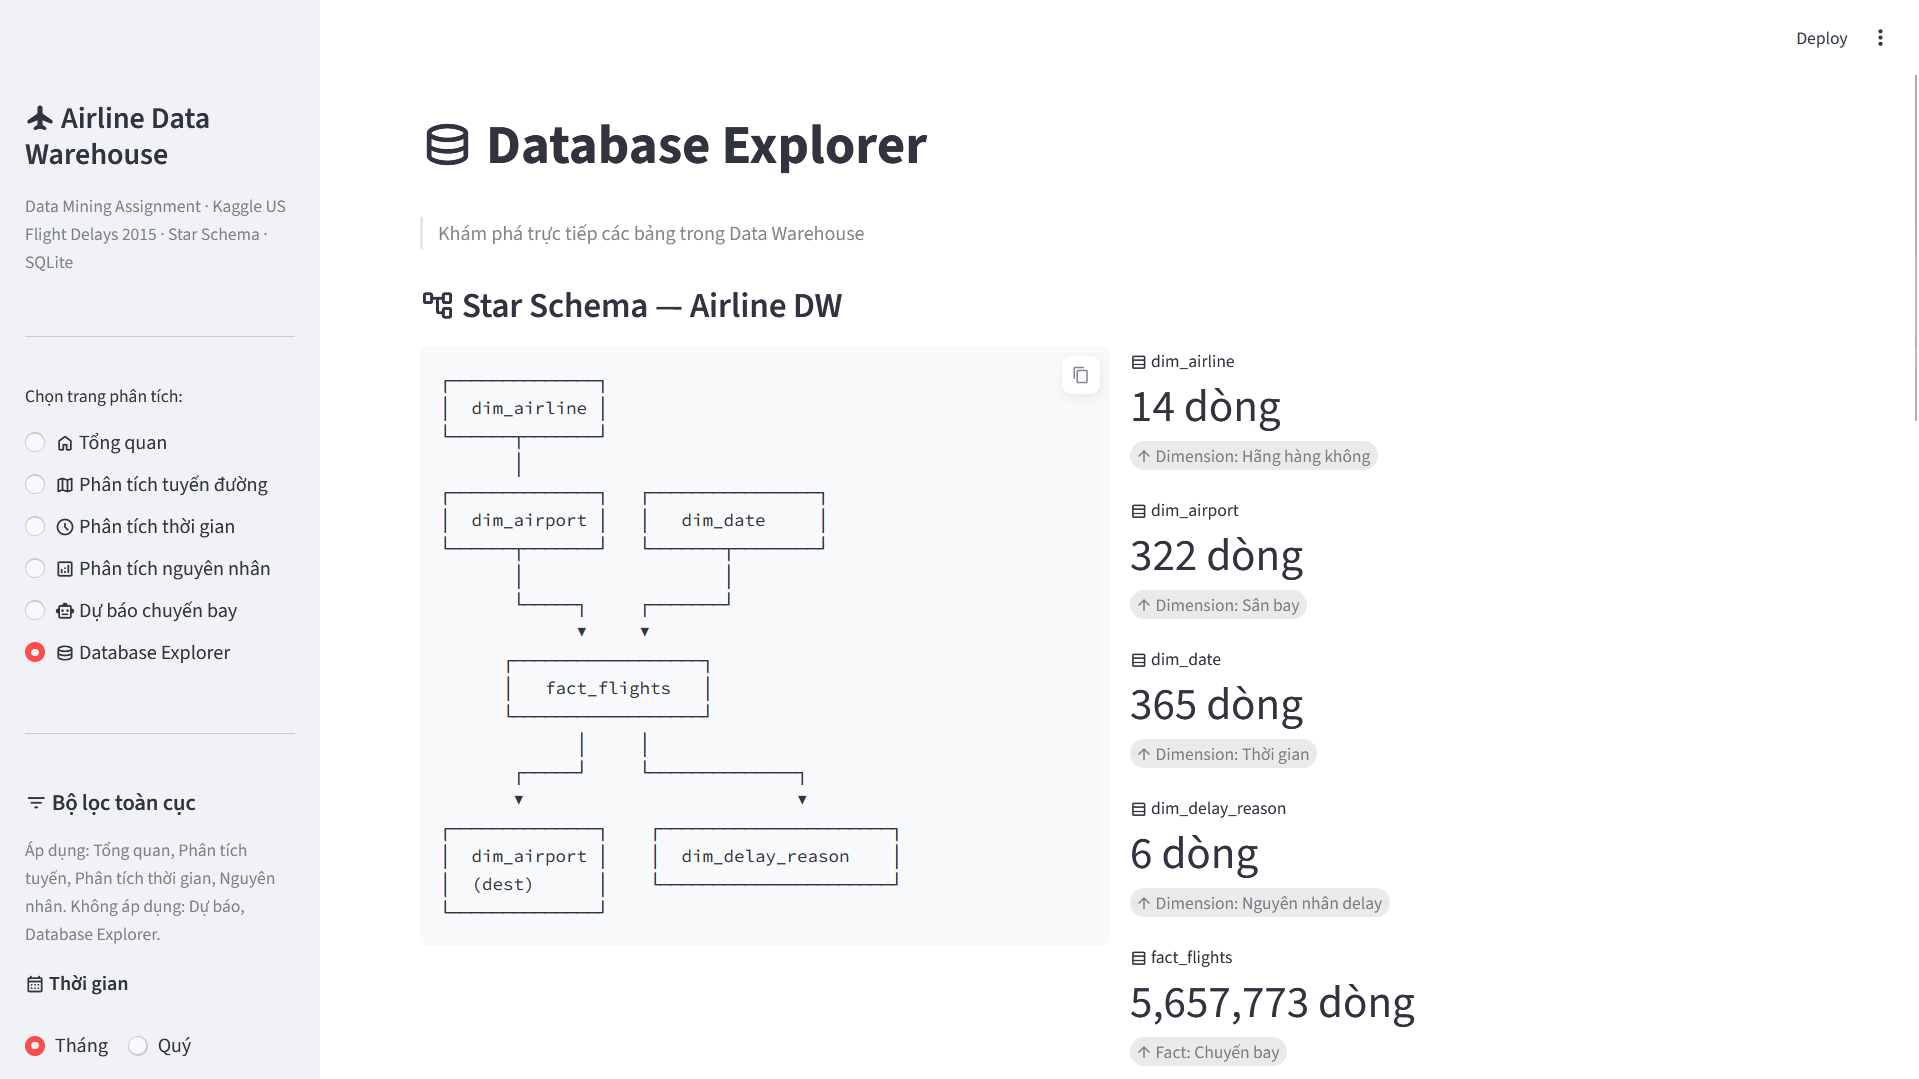
\includegraphics[width=\linewidth,height=0.48\textheight,keepaspectratio]{database.png}\\
\scriptsize Star schema ASCII, số dòng, xem trước bảng, SQL tùy chỉnh (chỉ SELECT).
\end{column}
\end{columns}
\end{frame}

% --- Slide 20 ---
\begin{frame}{Insight OLAP từ Dashboard}
Từ giao diện tương tác với dữ liệu năm 2015:

\begin{enumerate}
  \item \textbf{Tính mùa vụ rõ rệt:}
        Mùa hè (T6--T7) và mùa đông (T12--T1) là hai đỉnh delay.

  \item \textbf{Hiệu ứng tích lũy trong ngày:}
        Chuyến sáng sớm ($<$8h) ít delay nhất; chuyến tối chịu ảnh hưởng dây chuyền.

  \item \textbf{Chênh lệch giữa hãng:}
        OTP hãng tốt nhất vs. kém nhất chênh \textbf{15--20 điểm \%}.

  \item \textbf{Sân bay hub:}
        ORD, ATL, DFW có delay trung bình vượt mặt bằng chung.

  \item \textbf{Nguyên nhân chính:}
        NAS và Late Aircraft chiếm tỷ trọng trễ lớn nhất --- yếu tố \textit{hệ thống}.
\end{enumerate}
\end{frame}


% ================= SECTION 5: KHAI PHÁ DỮ LIỆU =================
% ============================================================
% SECTION 5: KHAI PHÁ DỮ LIỆU
% ============================================================
\section{Khai phá dữ liệu}

% --- Slide 21 ---
\begin{frame}{Phát biểu bài toán}
\begin{block}{Câu hỏi khai phá}
\textit{``Có thể dự đoán một chuyến bay sẽ trễ đến $\geq 15$ phút hay không,
chỉ dựa trên thông tin biết \textbf{trước} khi cất cánh?''}
\end{block}

\vspace{3mm}
\begin{columns}[T,onlytextwidth]
\begin{column}{0.5\textwidth}
\textbf{Bài toán phân lớp nhị phân:}
\begin{itemize}
  \item Nhãn: \texttt{is\_delayed\_15} (0/1).
  \item Mất cân bằng: 81\% / 19\%.
  \item \textbf{Không dùng} \texttt{departure\_delay}.
\end{itemize}
\end{column}
\begin{column}{0.5\textwidth}
\textbf{Quy trình end-to-end:}
\begin{enumerate}
  \item Lấy 500K mẫu (stratified theo tháng).
  \item Tiền xử lý + 10 đặc trưng.
  \item Holdout 80/20 (stratify=y).
  \item Huấn luyện 5 mô hình.
  \item Đánh giá 7 chỉ số.
\end{enumerate}
\end{column}
\end{columns}
\end{frame}

% --- Slide 22 ---
\begin{frame}{10 đặc trưng đầu vào}
\small
\begin{table}
\centering
\scriptsize
\begin{tabular}{clll}
\toprule
\textbf{Nhóm} & \textbf{Feature} & \textbf{Kiểu} & \textbf{Lý do} \\
\midrule
\multirow{4}{*}{\rotatebox{90}{\tiny Thời gian}}
  & \texttt{month}        & int   & Mùa vụ (bão hè, tuyết đông) \\
  & \texttt{day\_of\_week} & int   & Lưu lượng theo ngày \\
  & \texttt{is\_weekend}   & int   & Cờ cuối tuần \\
  & \texttt{quarter}       & int   & Quý trong năm \\
\midrule
\multirow{3}{*}{\rotatebox{90}{\tiny Chuyến}}
  & \texttt{dep\_hour}     & int   & Hiệu ứng tích lũy trong ngày \\
  & \texttt{distance}      & float & Quãng đường (dặm) \\
  & \texttt{elapsed\_time} & float & Thời gian bay (phút) \\
\midrule
\multirow{3}{*}{\rotatebox{90}{\tiny Ngữ cảnh}}
  & \texttt{airline\_enc}  & int   & Mã hãng (Label Encoding) \\
  & \texttt{origin\_enc}   & int   & Bang sân bay đi \\
  & \texttt{dest\_enc}     & int   & Bang sân bay đến \\
\bottomrule
\end{tabular}
\end{table}

\vspace{1mm}
\begin{alertblock}{Nguyên tắc quan trọng}
\small Loại \texttt{departure\_delay}, delay thành phần, \texttt{is\_cancelled}, \texttt{is\_diverted},
\texttt{tail\_number} --- tất cả chỉ biết \textit{sau} khi sự kiện xảy ra.
\end{alertblock}
\end{frame}

% --- Slide 23 ---
\begin{frame}{Cấu hình huấn luyện}
\small
\begin{table}
\centering
\scriptsize
\begin{tabular}{lp{8.5cm}}
\toprule
\textbf{Mô hình} & \textbf{Tham số chính} \\
\midrule
Logistic Regression & \texttt{saga}, C=1.0, \texttt{class\_weight='balanced'}, max\_iter=200 \\
Random Forest & 100 cây, max\_depth=10, min\_samples\_leaf=50, \texttt{class\_weight='balanced'} \\
Neural Network & [10$\to$64$\to$32$\to$1], ReLU, Adam, $\alpha$=0.001 (L2), batch=512, early stop \\
XGBoost & 300 cây, max\_depth=6, lr=0.05, subsample=0.8, \texttt{scale\_pos\_weight}$\approx$3.76 \\
LightGBM & 300 cây, max\_depth=6, lr=0.05, subsample=0.8, \texttt{is\_unbalance=True} \\
\bottomrule
\end{tabular}
\end{table}

\vspace{2mm}
\begin{block}{Xử lý mất cân bằng}
Dùng \textbf{trọng số lớp} (\texttt{class\_weight}, \texttt{scale\_pos\_weight}, \texttt{is\_unbalance})
thay vì over/undersampling $\to$ giữ nguyên phân phối gốc, tránh overfitting.
\end{block}
\end{frame}

% --- Slide 24 ---
\begin{frame}{Kết quả so sánh mô hình}
\small
\begin{table}
\centering
\begin{tabular}{lcccccc}
\toprule
\textbf{Mô hình} & \textbf{AUC} & \textbf{Acc.} & \textbf{F1} & \textbf{Avg.P} & \textbf{Log Loss} & \textbf{TG (s)} \\
\midrule
Logistic Regression & 0.6978 & 0.6570 & 0.6914 & 0.4120 & 0.6233 & \textbf{2.7} \\
Random Forest       & 0.7130 & 0.6375 & 0.6756 & 0.4107 & 0.6216 & 13.0 \\
Neural Network      & 0.7342 & \textbf{0.8318} & \textbf{0.7877} & 0.4809 & \textbf{0.4197} & 33.5 \\
XGBoost             & \textbf{0.7545} & 0.7054 & 0.7324 & \textbf{0.5078} & 0.5721 & 7.1 \\
LightGBM            & 0.7509 & 0.7031 & 0.7305 & 0.5014 & 0.5770 & 4.1 \\
\bottomrule
\end{tabular}
\end{table}

\vspace{2mm}
\begin{itemize}
  \item \textbf{XGBoost} dẫn đầu AUC-ROC (0,7545) và Avg. Precision (0,5078).
  \item \textbf{LightGBM} sát sau nhưng nhanh hơn đáng kể (4,1s vs. 7,1s).
  \item \textbf{Neural Network}: Accuracy/F1 cao nhất nhưng AUC thứ 3 --- thiên về lớp đa số.
\end{itemize}
\end{frame}

% --- Slide 25 ---
\begin{frame}{Confusion Matrix}
\centering
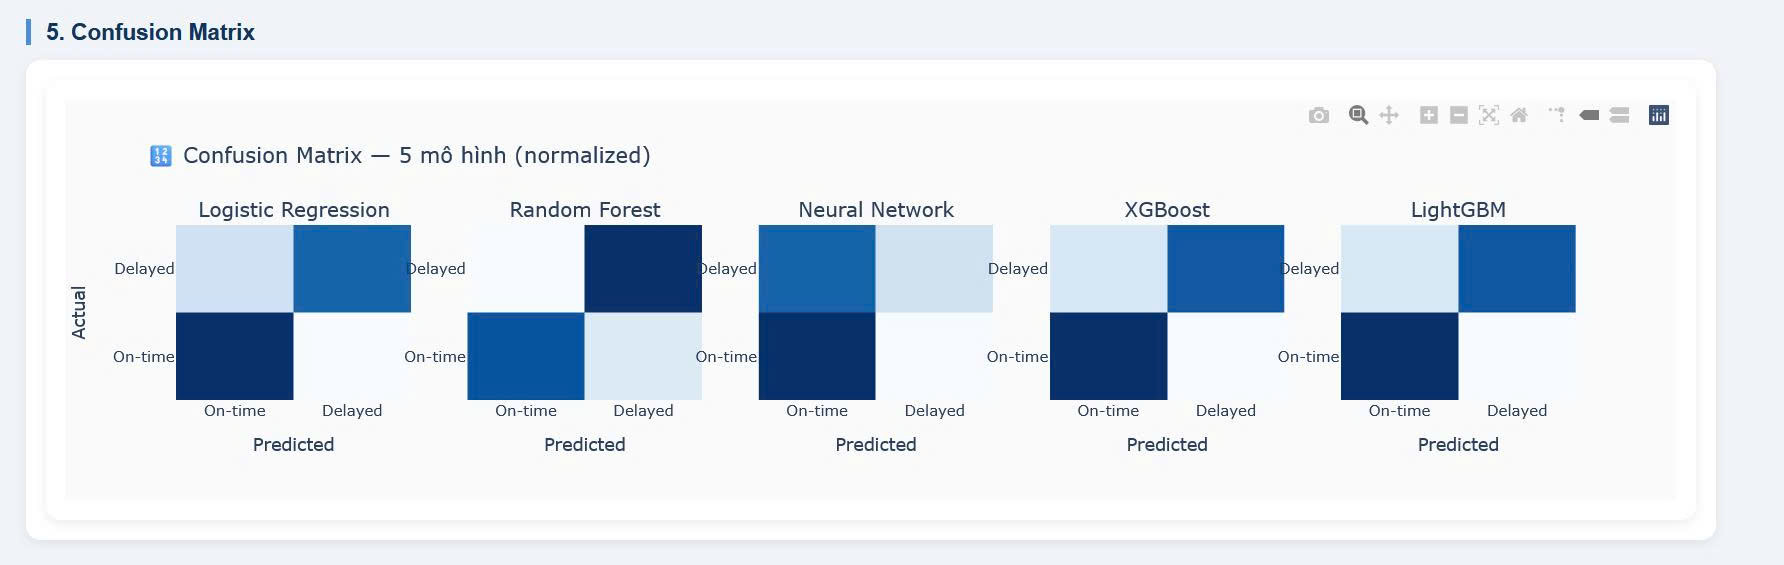
\includegraphics[width=\linewidth,keepaspectratio]{confusion_matrix.jpg}
\end{frame}

\begin{frame}{Confusion Matrix}
\textbf{LR \& RF:}\\
4 ô đồng đều --- chưa phân biệt rõ 2 lớp. AUC thấp nhất nhóm.

\vspace{2mm}
\textbf{Neural Network:}\\
True Negative rất đậm, nhưng False Negative cao $\to$ \textbf{bỏ sót delay}.
Accuracy 0,83 ``che giấu'' thiên lệch.

\vspace{2mm}
\textbf{XGBoost \& LightGBM:}\\
Đường chéo \textbf{cân đối nhất} --- phân biệt tốt \textit{cả hai lớp}.

\vspace{2mm}
\begin{alertblock}{}
\small Accuracy đơn thuần \textbf{gây hiểu nhầm} khi dữ liệu mất cân bằng.
\end{alertblock}
\end{frame}

% --- Slide 26 ---
\begin{frame}{Feature Importance}
\centering
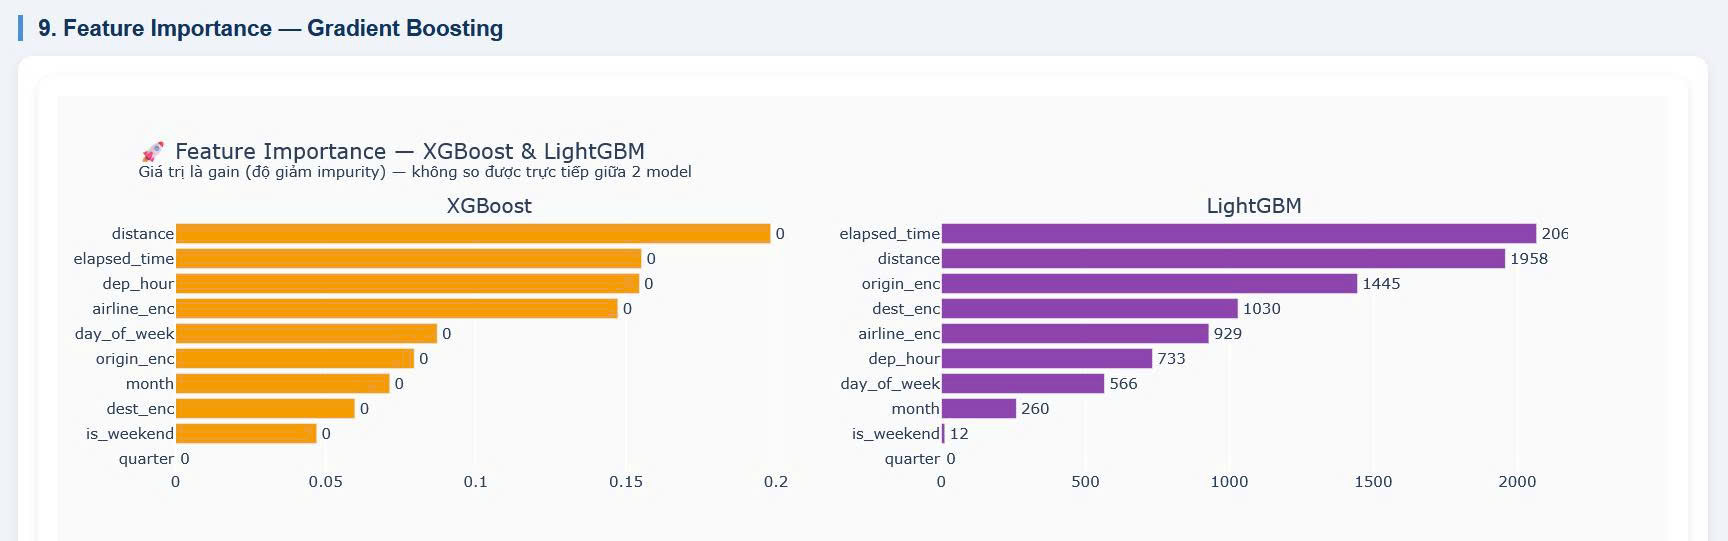
\includegraphics[width=\linewidth,keepaspectratio]{feature_importance.jpg}
\end{frame}

\begin{frame}{Feature Importance}
\textbf{Top features (cả 2 model):}
\begin{enumerate}
  \item \texttt{distance} \& \texttt{elapsed\_time}\\
        Chuyến dài = nhiều rủi ro hơn.
  \item \texttt{dep\_hour}\\
        Hiệu ứng tích lũy chiều/tối.
  \item \texttt{airline\_enc}\\
        OTP chênh 15--20\% giữa hãng.
  \item \texttt{origin/dest\_enc}\\
        Yếu tố địa lý quan trọng.
\end{enumerate}

\vspace{2mm}
\texttt{is\_weekend}, \texttt{quarter} thấp nhất
$\to$ đã ``bao hàm'' bởi \texttt{day\_of\_week}, \texttt{month}.

\vspace{2mm}
\textbf{Nhất quán với OLAP}: dashboard phát hiện xu hướng vĩ mô,
model lượng hóa đóng góp.
\end{frame}

% --- Slide 27 ---
\begin{frame}{Tại sao Gradient Boosting tốt nhất?}
\begin{enumerate}
  \item \textbf{Nắm bắt quan hệ phi tuyến}\\
        Delay vs. đặc trưng không tuyến tính --- LR không biểu diễn được.

  \item \textbf{Tự phát hiện interaction features}\\
        VD: hãng F9 + tháng 12 + sân bay ORD $\to$ delay cao.

  \item \textbf{Boosting tuần tự vs. Bagging song song}\\
        Mỗi cây sửa lỗi cây trước $\to$ hội tụ tốt hơn RF.

  \item \textbf{Xử lý mất cân bằng lớp tích hợp}\\
        \texttt{scale\_pos\_weight}, \texttt{is\_unbalance} điều chỉnh gradient theo tỷ lệ lớp.

  \item \textbf{LightGBM: tốc độ vượt trội}\\
        Leaf-wise + histogram: 4,1s vs. 7,1s, chỉ thua 0,004 AUC.
\end{enumerate}
\end{frame}

% --- Slide 28 ---
\begin{frame}{Những trường hợp mô hình còn sai}
Dù Gradient Boosting tốt nhất, AUC $\approx$ 0,75 vẫn còn khoảng cách:

\vspace{3mm}
\begin{columns}[T,onlytextwidth]
\begin{column}{0.48\textwidth}
\begin{block}{Nguyên nhân sai}
\begin{itemize}
  \item \textbf{Thời tiết cực đoan} đột xuất\\
        (bão tuyết, mưa đá bất ngờ).
  \item \textbf{Delay vận hành nội bộ}\\
        (thiếu phi hành đoàn, bảo trì đột xuất).
\end{itemize}
\end{block}
\end{column}
\begin{column}{0.48\textwidth}
\begin{block}{Nguyên nhân sai (tt.)}
\begin{itemize}
  \item \textbf{Sân bay/hãng ít dữ liệu}\\
        Encoding không đại diện.
  \item \textbf{Ngày lễ đặc biệt}\\
        Thanksgiving, Giáng sinh: hành vi delay khác biệt.
\end{itemize}
\end{block}
\end{column}
\end{columns}

\vspace{3mm}
$\Rightarrow$ Gợi ý: tích hợp dữ liệu thời tiết, thêm feature ngày lễ.
\end{frame}


% ================= SECTION 6: KẾT LUẬN =================
% ============================================================
% SECTION 6: KẾT LUẬN VÀ HƯỚNG PHÁT TRIỂN
% ============================================================
\section{Kết luận}

% --- Slide 29 ---
\begin{frame}{Insight từ dữ liệu 2015 \& Khuyến nghị}
\begin{enumerate}
  \item \textbf{Hiệu ứng dây chuyền là nguyên nhân delay lớn nhất}\\
        Late Aircraft + NAS chiếm tỷ trọng cao nhất.\\
        {\small\textit{$\to$ Tăng buffer thời gian quay đầu tàu bay tại hub.}}

  \item \textbf{Mùa hè (T6--T7) và mùa đông (T12--T1) = hai đỉnh delay}\\
        {\small\textit{$\to$ Phương án dự phòng riêng cho mùa cao điểm.}}

  \item \textbf{Chuyến sáng sớm ($<$8h) ít delay nhất}\\
        {\small\textit{$\to$ Ưu tiên chuyến sáng nếu cần đúng giờ.}}

  \item \textbf{Hãng bay ảnh hưởng có hệ thống:} chênh 15--20 điểm \% OTP.\\
        {\small\textit{$\to$ Benchmark OTP công khai tạo áp lực cải thiện.}}

  \item \textbf{distance, elapsed\_time, dep\_hour}: top feature importance.\\
        {\small\textit{$\to$ Chuyến dài + chiều/tối = rủi ro cao nhất.}}
\end{enumerate}
\end{frame}

% --- Slide 30 ---
\begin{frame}{Đánh giá hoàn thành mục tiêu}
\begin{table}
\centering
\small
\begin{tabular}{clc}
\toprule
\textbf{\#} & \textbf{Mục tiêu} & \textbf{Kết quả} \\
\midrule
1 & Data Warehouse chuẩn hóa & \textcolor{green!60!black}{\ding{51}} Star Schema, 5,3M bản ghi, ETL 3--8 phút \\
2 & Dashboard OLAP đa trang & \textcolor{green!60!black}{\ding{51}} 6 trang, Slice/Dice/Roll-up/Drill-down \\
3 & Mô hình dự báo delay & \textcolor{green!60!black}{\ding{51}} XGBoost AUC 0,7545 (best), 5 models so sánh \\
\bottomrule
\end{tabular}
\end{table}

\vspace{3mm}
\begin{block}{Giá trị hệ thống}
Không chỉ trực quan hóa dữ liệu lịch sử, hệ thống còn \textbf{hỗ trợ ra quyết định}
bằng mô hình dự báo delay \textbf{trước cất cánh}.
\end{block}
\end{frame}

% --- Slide 31 ---
\begin{frame}{Hạn chế}
\begin{enumerate}
  \item \textbf{Dữ liệu chỉ bao phủ năm 2015}\\
        Mô hình có thể không phù hợp với thực tế sau COVID-19.
        Tuy nhiên \textit{phương pháp luận} vẫn áp dụng được khi đổi nguồn dữ liệu.

  \item \textbf{SQLite không phù hợp production}\\
        Single-writer, không concurrent access, một số OLAP query mất vài giây.

  \item \textbf{AUC $\approx$ 0,75 --- còn khoảng cách}\\
        Thiếu dữ liệu thời tiết, bảo trì, lịch sử delay từng tail number.

  \item \textbf{Chưa có Clustering / Association Rules}\\
        Chỉ tập trung classification và OLAP.
\end{enumerate}
\end{frame}

% --- Slide 32 ---
\begin{frame}{Hướng phát triển}
\begin{columns}[T,onlytextwidth]
\begin{column}{0.48\textwidth}
\begin{block}{Dữ liệu \& Mô hình}
\begin{enumerate}
  \item Mở rộng dữ liệu 2010--2023 (BTS).
  \item Tích hợp thời tiết NOAA.
  \item Thêm feature ngày lễ.
  \item SHAP giải thích từng dự báo.
\end{enumerate}
\end{block}
\end{column}
\begin{column}{0.48\textwidth}
\begin{block}{Hạ tầng \& Triển khai}
\begin{enumerate}
  \item PostgreSQL / ClickHouse thay SQLite.
  \item Docker + Cloud deploy.
  \item REST API (FastAPI) cho dự báo real-time.
  \item Apache Kafka + Spark Streaming.
\end{enumerate}
\end{block}
\end{column}
\end{columns}
\end{frame}

% --- Slide cuối ---
\setbeamertemplate{footline}{}

\begin{frame}
    \centering
    \vspace{1cm}
    \textbf{\Huge{- THE END - }}\\
    \vspace{0.2cm}
    \textit{\Large{Cảm ơn thầy đã lắng nghe phần trình bày của nhóm em}}\\
    \vspace{15pt}
    \begin{columns}
        \begin{column}{0.4\textwidth}
            \centering
            
\includegraphics[width=0.8\textwidth]{paper.jpg}
        \end{column}
        \begin{column}{0.6\textwidth}
            \centering
            Kính chúc thầy luôn mạnh khỏe, nhiều niềm vui và luôn giữ được ngọn lửa đam mê với nghề.
        \end{column}
    \end{columns}
\end{frame}


\end{document}
